Since the beginning of time, humans were getting to know their environment. It did not take long, until the first humans started getting even further and become explorers. They started leaving marks and using landmarks to remember pathways and places. This primitive representation of prehistoric places and early history maps can be traced back to 24000-25000 BC. Soon after, they started using maps which revolutionized the way we navigate and the way we travel, and therefore the field of Cartography become a reality. During the 19th century terra incognita disappeared from maps, since both the coastlines and the inner parts of the continents had been fully explored. Today, using technology and satellites, Earth is completely mapped, yet not completely explored.


\begin{figure}[!htb]
	\centering
	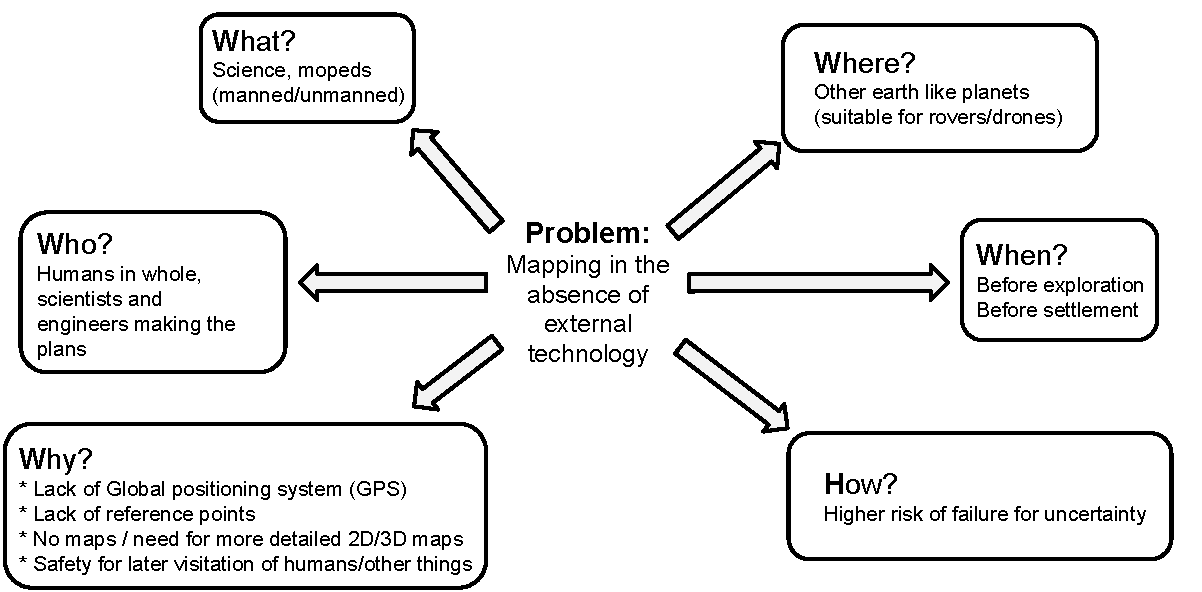
\includegraphics[scale=.7]{images/wdiagram1.pdf}
	\caption{W-diagram}
	\label{fig:wdiagram}
\end{figure}

%http://wwws.phil.uni-passau.de/histhw/tutcarto/english/index-frames-en.html
%http://www.e-perimetron.org/Vol_2_2/Wolodchenko_Forner.pdf
%http://en.wikipedia.org/wiki/Terra_incognita
%http://en.wikipedia.org/wiki/History_of_cartography